\chapter{Analisi della letteratura}
\label{chap:2}

    \paragraph{Dizionario dei termini}
        In questo paragrafo, si illustrano i termini tecnici comunemente utilizzati nella letteratura per descrivere gli adversarial attacks applicati al deep learning in Computer Vision:
            \begin{itemize}
                \item \textbf{Adversarial example/image} (Immagine/esempio avversario): è una versione modificata di un'immagine pulita che viene intenzionalmente perturbata (ad esempio aggiungendo del rumore) per confondere/ingannare una tecnica di apprendimento automatico, come le DNN.
                \item \textbf{Adversarial perturbation/noise} (Perturbazione avversaria/rumore): è il rumore che viene aggiunto ad un'immagine pulita per renderla un adversarial example.
                \item \textbf{Adversary} (Avversario): si riferisce più comunemente all'agente che crea un esempio avversario.
                \item \textbf{Modello/classificatore/algoritmo di classificazione}: è l'algoritmo che prende in input un'immagine e la riconosce restituendo in output la sua etichetta/classe. È la tecnica di apprendimento automatico che analizza l'immagine e la classifica.
            \end{itemize}

\section{Adversarial Attacks}
Nella figura \ref{Panda}, è possibile vedere come l'immagine iniziale venga classificata correttamente come un panda mentre, con l'aggiunta di un rumore molto piccolo, il modello classifichi con sicurezza il panda come un gibbone.
    \begin{figure}[!h]
        \centering
        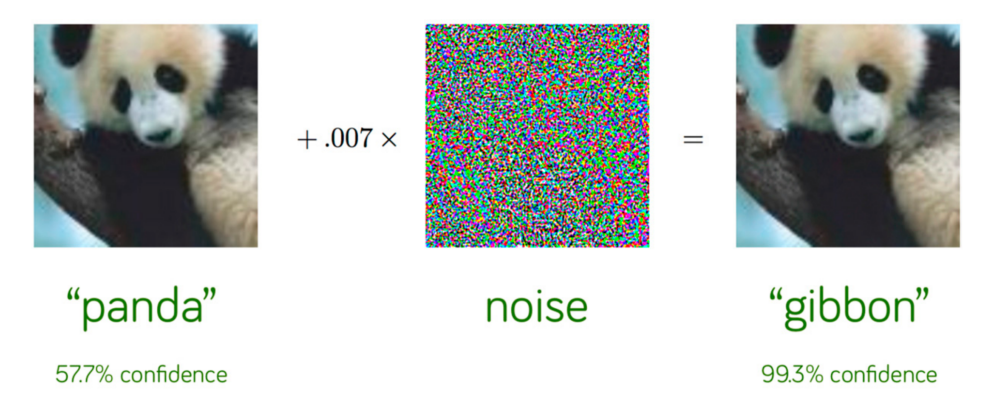
\includegraphics[width=0.7\textwidth]{Images/Panda.png}
        \caption{Previsione del modello prima e dopo l'attacco.}
        \label{Panda}
    \end{figure}

Le prime spiegazioni sugli adversarial attacks riguardavano la non linearità e l'overfitting mentre, successivamente, Goodfellow %[https://arxiv.org/pdf/1412.6572.pdf] 
\cite{goodfellow2014explaining} ha dimostrato che %la ragione di tale vulnerabilità è proprio la linearità dei modelli.
anche i modelli lineari erano altamente vulnerabili.
Anche altri studi hanno cercato di spiegare questo fenomeno. Schmid %[https://arxiv.org/pdf/1804.11285.pdf] 
\cite{schmidt2018adversarially} sostiene che il successo degli adversarial attacks sia dovuto alla carenza di dati reali e alla loro distribuzione non omogenea. Ilyas %[https://arxiv.org/pdf/1905.02175.pdf] 
\cite{ilyas2019adversarial} afferma che questi attacchi sono efficaci a causa delle capacità di generalizzazione dei modelli su un dataset specifico: il modello estrae così features altamente prevedibili ma non robuste.\\

Finora, la maggior parte degli studi esistenti sono stati effettuati su immagini naturali. Le immagini naturali hanno numerose differenze rispetto alle immagini mediche e questo è un motivo fondamentale per studiare come gli adversarial attacks influenzano le immagini mediche.

Prima di tutto, si ha un'insufficienza di grandi datasets di immagini mediche con etichette annesse a causa dell'elevato costo e del consumo di tempo che comporta la raccolta dei dati. Inoltre, la classe normale è spesso sovrarappresentata, portando quindi ad una convergenza lenta e al problema dell'overfitting.

Un'altra differenza tra questi due tipi di immagini è che i dati medici spesso contengono informazioni quantitative mentre le immagini naturali no. 

Inoltre, ci sono munerosi casi in cui le differenze tra le classi sono molto piccole.
Ad esempio, una radiografia con una polmonite allo stadio iniziale è abbastanza simile ad una radiografia normale. 

In aggiunta, le immagini naturali sono generate da telecamere RGB, mentre la maggior parte delle immagini mediche non lo sono. 

Tuttavia, numerosi studi hanno dimostrato che anche le immagini mediche possono essere influenzate da adversarial attacks. %[https://www.medrxiv.org/content/10.1101/2021.01.17.21249704v1.full, https://www.ncbi.nlm.nih.gov/pmc/articles/PMC7738012/, https://www.sciencedirect.com/science/article/pii/S1361841521001870?via%3Dihub#sec0010].
Ad esempio le immagini oncologiche \cite{joel2021adversarial}, le immagini dermatologiche \cite{allyn2020adversarial} e le fondoscopie \cite{bortsova2021adversarial}.

Ma è stato provato %[https://arxiv.org/pdf/1907.10456.pdf] 
\cite{ma2021understanding} che i modelli DL medici sono più vulnerabili dei modelli di immagini naturali per due motivi: 
    \begin{enumerate}
        \item la caratteristica texture biologica delle immagini mediche ha molte aree che possono essere facilmente ingannate;
        \item i moderni modelli DL sono costituiti da molti livelli in quanto sono stati progettati per l'elaborazione delle immagini naturali. Introducono quindi un elevato numero di parametri che, nel caso dell'analisi delle immagini mediche, può portare ad una iper-parametrizzazione ed aumentare la vulnerabilità del modello.
    \end{enumerate}

Nonostante ciò, gli attacchi nelle immagini mediche sono rilevati più facilmente che in un'immagine naturale, poiché le caratteristiche avversarie sono linearmente separate dalle caratteristiche normali, mentre nelle immagini naturali gli adversarial examples sono simili ai normali.

\newpage

\section{Mitigation di Adversarial Attacks}
Al fine di ridurre la vulnerabilità dei modelli DL, nel corso degli ultimi anni sono state studiate numerose tecniche di difesa per mitigare gli adversarial attacks.

\paragraph{Input Denoising}
Poiché un adversarial attack consiste nell'aggiungere ai dati un rumore impercettibile all'occhio umano, allora una soluzione di difesa naturale potrebbe essere quella di provare ad eliminare la perturbazione.

Formalmente, dati un'immagine pulita $x$, il rispettivo adversarial example $x_{adv}$ e un modello di classificazione $f$, si cerca di progettare una mappatura $f_m$ tale che $f(f_m(x_{adv})) = f(x)$.

Recentemente sono state sviluppate delle difese che ricorrono a schemi di randomizzazione per eliminare le perturbazioni avversarie. 

L'intuizione dietro questo tipo di difesa è che le DNN sono da sempre robuste alle perturbazioni casuali. Una difesa basata sulla randomizzazione cerca di randomizzare i rumori avversari in rumori casuali, che non sono una preoccupazione per la maggior parte delle DNN. 
\\

Tra queste tecniche troviamo il Feature Squeezing \cite{xu2017feature}, che consiste nell'utilizzo di due metodi di squeezing, riduzione dei bit e sfocatura dell'immagine. 
Il rilevamento dell'adversarial example è realizzato confrontando le previsioni del modello sulle immagini originali e quelle prodotte dagli squeezing. Se i due input passati al modello producono output sensibilmente diversi, è probabile che l'input originale sia un adversarial example. Nonostante il Feature Squeezing risulti una tecnica di difesa molto efficace contro attacchi potenti come C\&W (Carlini \& Wagner), è stato dimostrato \cite{he2017adversarial, sharma2018bypassing} che è ancora troppo vulnerabile.
\\

Un altro modo per riportare le immagini al loro stato iniziale è l'impiego delle Generative Adversarial Networks (GANs).
Una GAN è un potente strumento in grado di apprendere un modello generativo per le distribuzioni di dati. Per questo molti studi le sfruttano per apprendere distribuzioni di dati puliti al fine di generare, per ogni adversarial example, la rispettiva controparte pulita. 

Due esempi sono Defense-GAN \cite{samangouei2018defense} e Adversarial perturbation elimination GAN (APE-GAN) \cite{shen2017ape}. 

Defense-GAN traina un generatore per modellare la distribuzione delle immagini pulite. Durante la fase di testing, Defense-GAN elimina la perturbazione avversaria cercando un'immagine vicina all'adversarial example in input nella distribuzione appresa. Restituisce quindi un'immagine pulita che darà in input al classificatore.
Questa strategia può essere utilizzata per difendersi da vari adversarial attacks, ma non tutti. Attualmente, lo schema di attacco più efficace contro Defense-GAN è basato su una tecnica chiamata \textit{Backward
Pass Differentiable Approximation} \cite{athalye2018obfuscated}, ed è in grado di ridurre la sua precisione fino al 55\%. 

APE-GAN traina direttamente un generatore per pulire un adversarial example, preso in input, e genera una controparte pulita. Anche se APE-GAN raggiunge buoni risultati \cite{shen2017ape}, l'attacco white-box proposto da Carlini e Wagner \cite{carlini2017magnet} può facilmente sconfiggerla. 

\paragraph{Model Robustification}
Un'altra strategia ampiamente adottata consiste nel raffinare il modello per prepararsi ad affrontare una potenziale minaccia.
Il perfezionamento del modello potrebbe essere ottenuto in due modi: cambiando l'obiettivo della fase di training o modificando la struttura del modello.
\\

Nel primo caso, l'idea di base è quella di considerare la minaccia degli adversarial attacks e rendere il modello più robusto durante la fase di training. 

Una di queste tecniche è l'Adversarial Training \cite{goodfellow2014explaining}, durante il quale il modello viene addestrato con immagini pulite e perturbate, entrambe etichettate correttamente.
\\

Esempi di modifica del modello includono la Model Distillation \cite{papernot2015distillation}, che utilizza le conoscenze del modello per migliorare la propria robustezza. Le conoscenze vengono estratte sotto forma di vettori di classi di probabilità dei dati di training e vengono date in input al modello originale per trainarlo nuovamente.
\\

Formalmente, dati un'immagine pulita $x$, il rispettivo adversarial example $x_{adv}$, la rispettiva classe $y$ e un modello di classificazione $f$, si cerca di progettare un modello robusto $f'$, basato su $f$, tale che $f'(x_{adv}) = f'(x) = y$.


\paragraph{Adversarial Detection}
Nelle due strategie precedenti, data un'istanza $x$, si cerca di predire la sua vera classe. L'Adversarial Detection, invece, mira a stabilire se un'istanza data è un adversarial examples.

Formalmente, data un'immagine $x'$, si cerca di progettare un modello $f_d$ tale che $f_d(x') = 1$ se e solo se $x'$ è un adversarial examples, altrimenti $f_d(x') = 0$.
\\

Una tecnica di difesa di questo tipo è MagNet \cite{meng2017magnet}, che include un detector ed un reformer, ed utilizza un autoencoder per imparare la distribuzione dei campioni puliti. Il detector distingue i campioni puliti e quelli avversari in base alle relazioni tra questi campioni e la distribuzione appresa. Il reformer è progettato per rettificare gli adversarial examples in campioni puliti. MagNet risulta efficace contro una varietà di adversarial attacks sotto impostazioni gray-box e black-box, come FGSM, BIM, e C\&W. Tuttavia, Carlini e Wagner \cite{carlini2017magnet} dimostrano che MagNet è vulnerabile agli adversarial examples trasferibili generati da un attacco.